\documentclass[a4paper]{article}

\usepackage[english]{babel}
\usepackage[utf8]{inputenc}
\usepackage{amsmath}
\usepackage{graphicx}
%\usepackage[colorinlistoftodos]{todonotes}

\usepackage{amsmath}
\DeclareMathOperator*{\argmax}{arg\,max}
\DeclareMathOperator*{\argmin}{arg\,min}

\title{Elaborazione di dati tridimensionali: homework 2}

\author{Alberto Cenzato 1134707}

\date{\today}

\begin{document}
\maketitle

\begin{abstract}
Scopo di questo secondo homework era di familiarizzare con la libreria PCL. Sono stati svolti quattro esercizi di complessità crescente per approfondire diverse funzionalità di PCL: lettura di point cloud da file, lettura e visualizzazione dei valori contenuti nella point cloud, downsampling, calcolo di normali, keypoint e descrittori, registrazione di point cloud, people detection.
\end{abstract}

\section{Lab 1} \label{sec:lab1}
La prima esperienza era suddivisa in due esercizi. Nel primo lo scopo era di rimuovere dalla point cloud tutti i punti con $X > 0$ e colorare i rimanenti in blu. Nel secondo era necessario filtrare la point cloud facendo di fatto un downsample dell'immagine 3D con risoluzioni diverse per ogni quadrante del piano $X$-$Y$.

	\subsection{Algortimi utilizzati}
	Per quanto riguarda il primo esercizio non c'è molto da dire sugli algoritmi utilizzati. Infatti, per modificare il colore dei punti, è sufficiente iterare su tutti i punti, verificare se $X > 0$ e in caso affermativo copiare il punto in una nuova point cloud modificando il suo colore in blu. La nuova cloud sarà quindi definita $C' = \left\{p \in C | p.x > 0, p.b = 255 \right\}$.
	Per filtrare la point cloud invece è stata usata la classe di PCL \verb|VoxelGrid| che divide lo spazio 3D in voxel: tutti i punti all'interno di un voxel vengono approssimati col loro centroide. Modificando la dimensione degli spigoli dei voxel si ottiene un donwsample maggiore o minore.
	
	\subsection{Considerazioni}
	L'implementazione è stata piuttosto diretta a partire dai file di esempio forniti, sono state necessarie solo alcune modifiche. L'output del secondo esercizio è mostrato in figura \ref{fig:lab1} 
	
	\begin{figure}
		\centering
		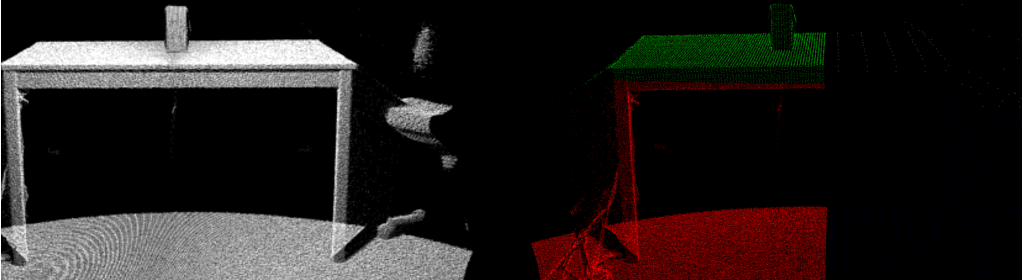
\includegraphics[width=1\textwidth]{images/lab1.png}
		\caption{\label{fig:lab1}Esempio di point cloud filtrata e colorata: a sinistra l'originale, a destra l'output.}
	\end{figure}


\section{Lab 2} \label{sec:lab2}
I due esercizi della seconda esperienza puntavano a calcolare le normali ad una superficie definita da una point cloud e ad utilizzare queste normali per il calcolo di features che possano essere caratteristiche e univoche per ogni punto.

	\subsection{Algortimi utilizzati}
	Il calcolo delle normali è stato fatto attraverso la classe di PCL \verb|NormalEstimationOMP|. \verb|NormalEstimationOMP| per ogni punto $p$ cerca i suoi vicini all'interno di una sfera di raggio $r$, questi vengono usati per stimare il piano $\pi^*$ che meglio approssima la superficie nel punto $p$; cioè si calcola 
	
	\begin{equation}
	\pi^* = \argmin{\sum_{x_i \in kNN(p)}{dist(x_i,\pi)}}
	\end{equation}
	
	\verb|NormalEstimationOMP| utilizza OpenMP per fornire un'implementazione multithread multipiattaforma. \\
	Vengono poi identificati i keypoint della point cloud, punti che per caratteristiche di posizione e/o colore rispetto ai loro vicini possono essere considerati salienti. Un buon keypoint detector dovrebbe essere invariante per traslazione, rotazione, scala e lumiosità, identificando sempre gli stessi keypoint indipendentemente dalle trasformazioni a cui viene sottoposta la point cloud. Per questo esercizio è stato scelto \verb|SIFT3D|, un'estensione di \verb|SIFT| in tre dimensioni, implementato dalla classe PCL \verb|SIFTKeypoint|. \\
	Una volta identificati i keypoint questi devono poter essere descritti o comparati in qualche modo. A questo scopo si utilizzano dei feature vector, cioè ad ogni keypoint viene assegnato un vettore caratteristico che identifica in modo univoco quel punto. Il contenuto dal vettore dipende dal feature descriptor utilizzato; per questo esercizio è stato usato \verb|Fast Point Feature Histogram|. L'algoritmo considera il keypoint e tutti i suoi vicini entro un raggio $r$; per ogni coppia dell'insieme vengono calcolati i tre angoli che definiscono l'orientazione reciproca delle due normali; infine crea un istogramma a partire dalle orientazioni di tutte le coppie. Il feature vector così estratto è invariante per rotazione e traslazione della point cloud.

	\subsection{Considerazioni}
	Il calcolo delle normali e l'estrazione delle features è piuttosto semplice grazie alle classi di PCL. La parte più lunga, come spesso accade con questi algoritmi, è la taratura dei parametri migliori per ottenere il risultato desiderato. Per \verb|SIFTKeypoint| sono stati usati \verb|min_scale = 0.01|, \verb|n_octaves = 3|, \verb|n_scales_per_octave = 4|, \verb|min_contrast = 0.001|. In figura \ref{fig:lab2} si possono vedere due esempi di descrittori calcolati con \verb|FPFHEstimationOMP|.
	
	\begin{figure}
		\centering
		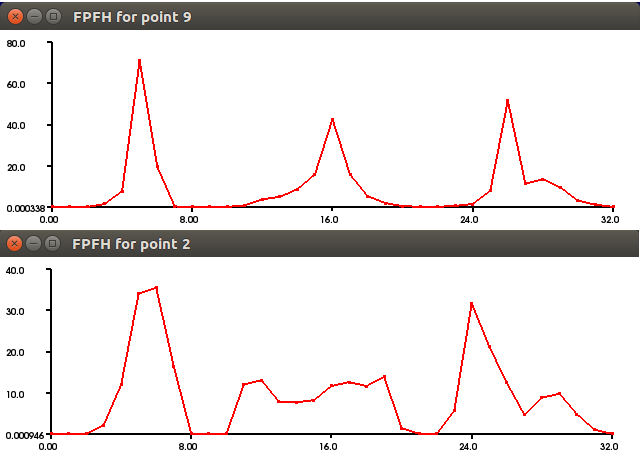
\includegraphics[width=1\textwidth]{images/lab2.png}
		\caption{\label{fig:lab2}Due esempi di descrittori FPFH per due keypoint diversi.}
	\end{figure}


\section{Lab 3} \label{sec:lab3}
Descrizione bla bla

	\subsection{Algortimi utilizzati (teoria)}

	\subsection{Considerazioni}


\section{Lab 4} \label{sec:lab4}
Descrizione bla bla

	\subsection{Algortimi utilizzati (teoria)}


	\subsection{Considerazioni}


\begin{thebibliography}{9}
\bibitem{nano3}
  K. Grove-Rasmussen og Jesper Nygård,
  \emph{Kvantefænomener i Nanosystemer}.
  Niels Bohr Institute \& Nano-Science Center, Københavns Universitet

\end{thebibliography}
\end{document}